\section{position}\label{position}

ADD $1/N_TEL$ LINE TO THE RES/MULTI PLOTS AND COMPARE WITH RESULTS
MENTIONED HERE:
\url{https://arxiv.org/pdf/astro-ph/9904234.pdf}

\subsection{Analysis at telescope level}

The random forests for the DISP- and SIGN-prediction get trained on
XXX diffuse gamma events with a 3-fold cross-validation.
The SIGN-model is not needed for this part, but can be useful as 
a cross-check for the LST-mono analysis in section \ref{lst mono part}.

The performance of the models can be gauged by looking at the 
figures \ref{fig:disp_test_perf} for the cross-validated set and 
\ref{fig:disp_test_perf} for the performance our 
pointlike data.

In both cases we can see that the DISP-model gets rapidly more
powerful with higher energies up until ~\SI{1}{\tera\electronvolt} from 
where on the performance stays the same.

The SIGN-model does not saturate like this and improves pretty linear up until
the highest energies.

\begin{figure}
    \begin{subfigure}{0.45\textwidth}
        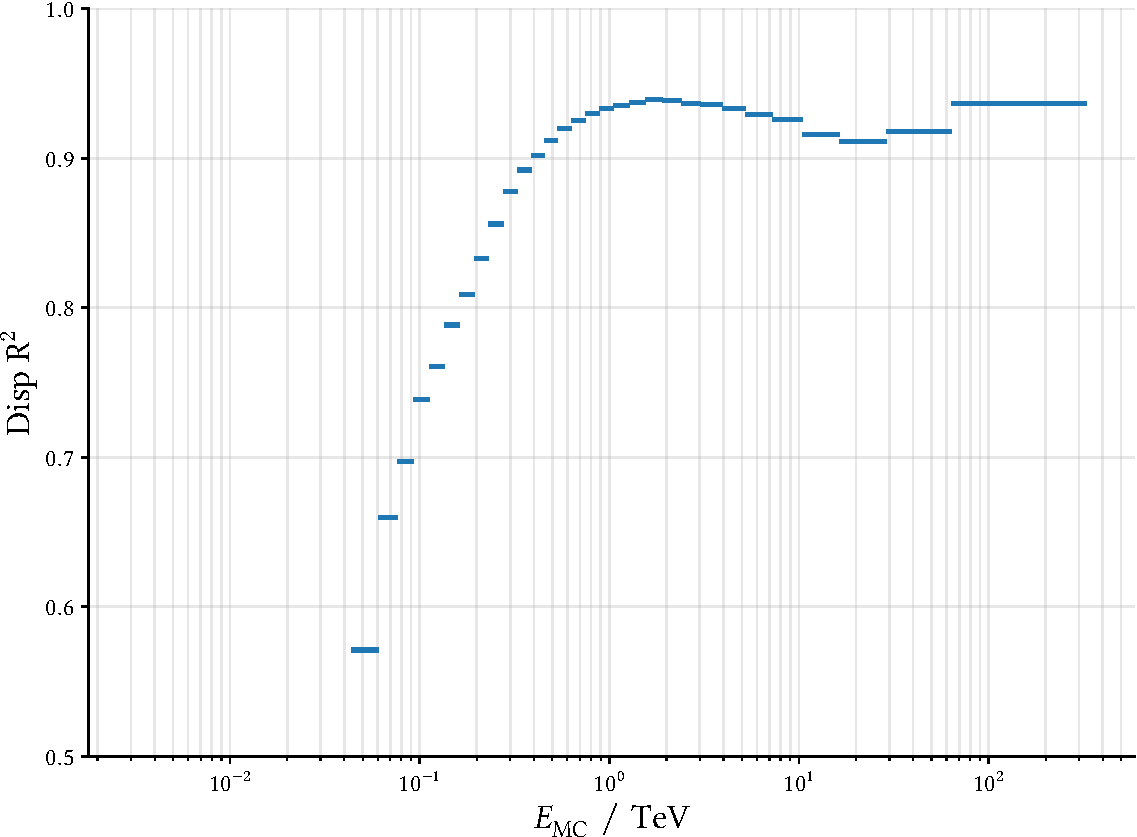
\includegraphics[width=0.9\linewidth]{../analysis/plots/disp_test_r2_equal_filled.pdf} 
        \caption{R2-Score for the DISP-estimation}
    \end{subfigure}
    \begin{subfigure}{0.45\textwidth}
        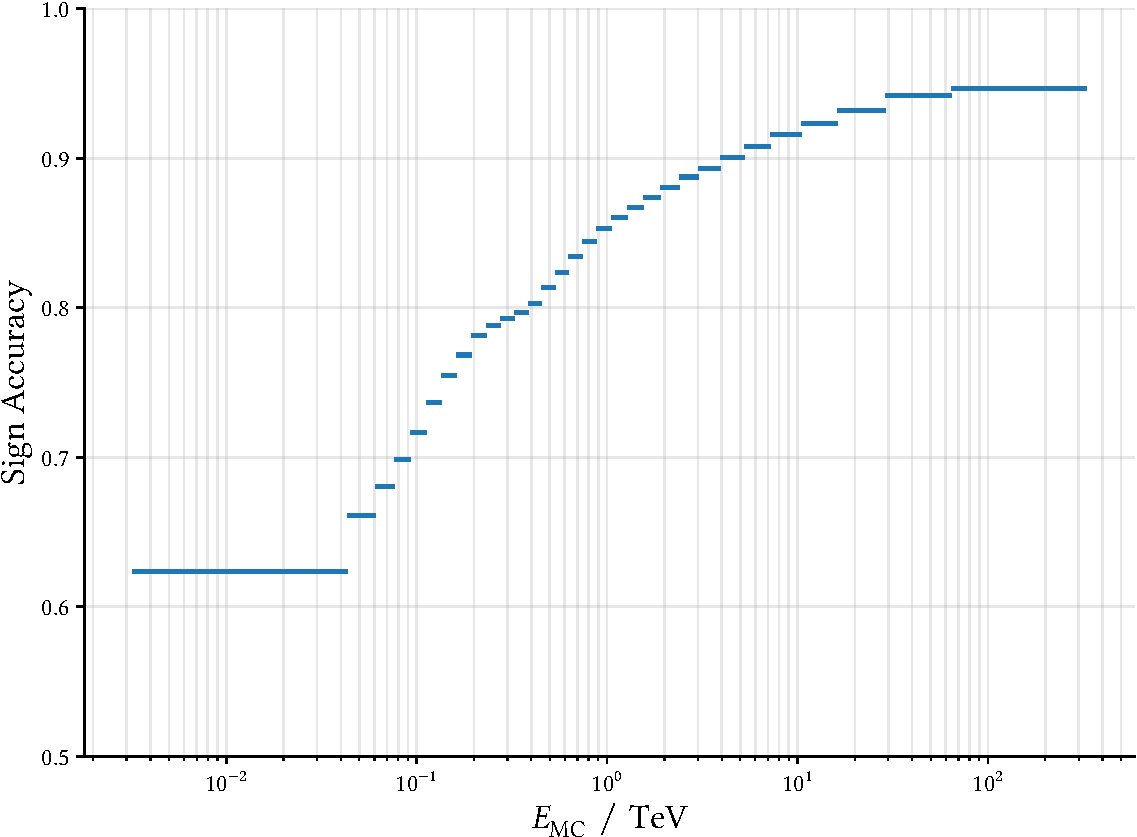
\includegraphics[width=0.9\linewidth]{../analysis/plots/disp_test_acc_equal_filled.pdf}
        \caption{SIGN-accuracy}
    \end{subfigure}
    \caption{Performance of the DISP- and SIGN-estimation algorithm on the test-dataset.}
    \label{fig:disp_test_perf}
\end{figure}

\begin{figure}
    \begin{subfigure}{0.45\textwidth}
        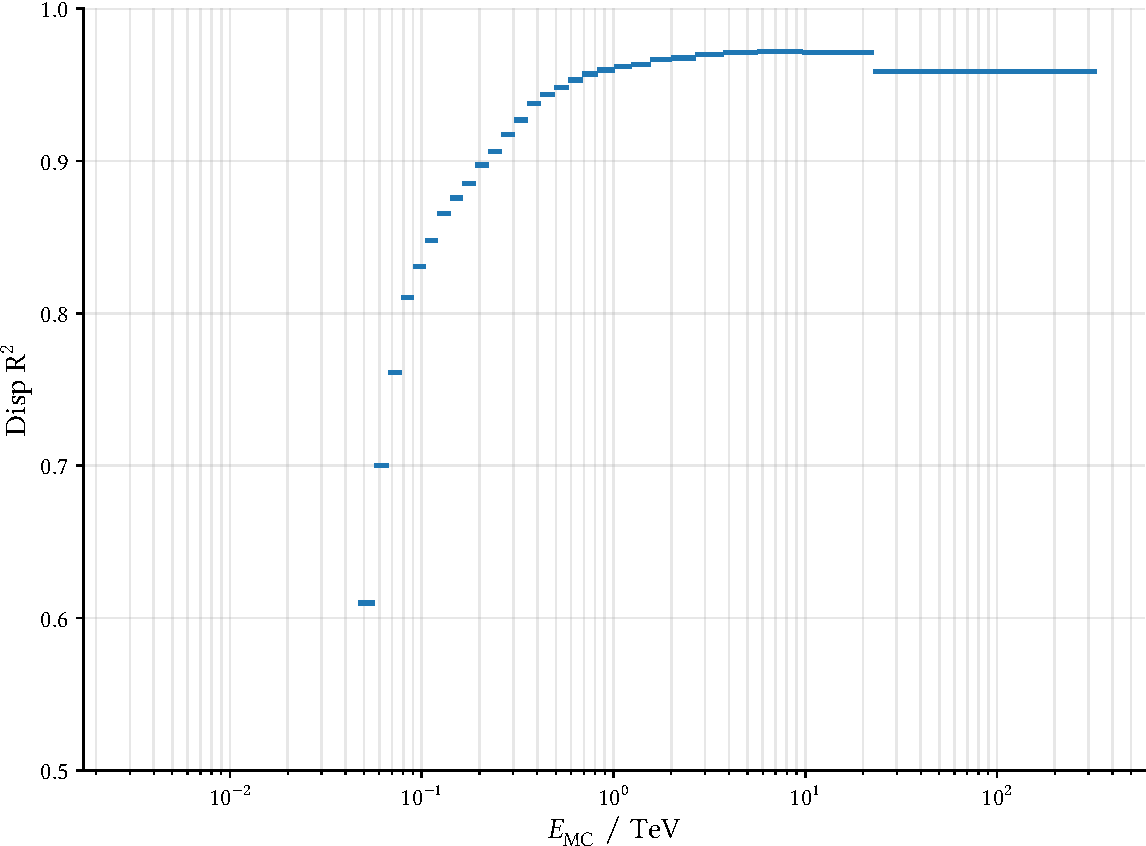
\includegraphics[width=0.9\linewidth]{../analysis/plots/disp_gamma_r2_equal_filled.pdf} 
        \caption{R2-Score for the DISP-estimation}
    \end{subfigure}
    \begin{subfigure}{0.45\textwidth}
        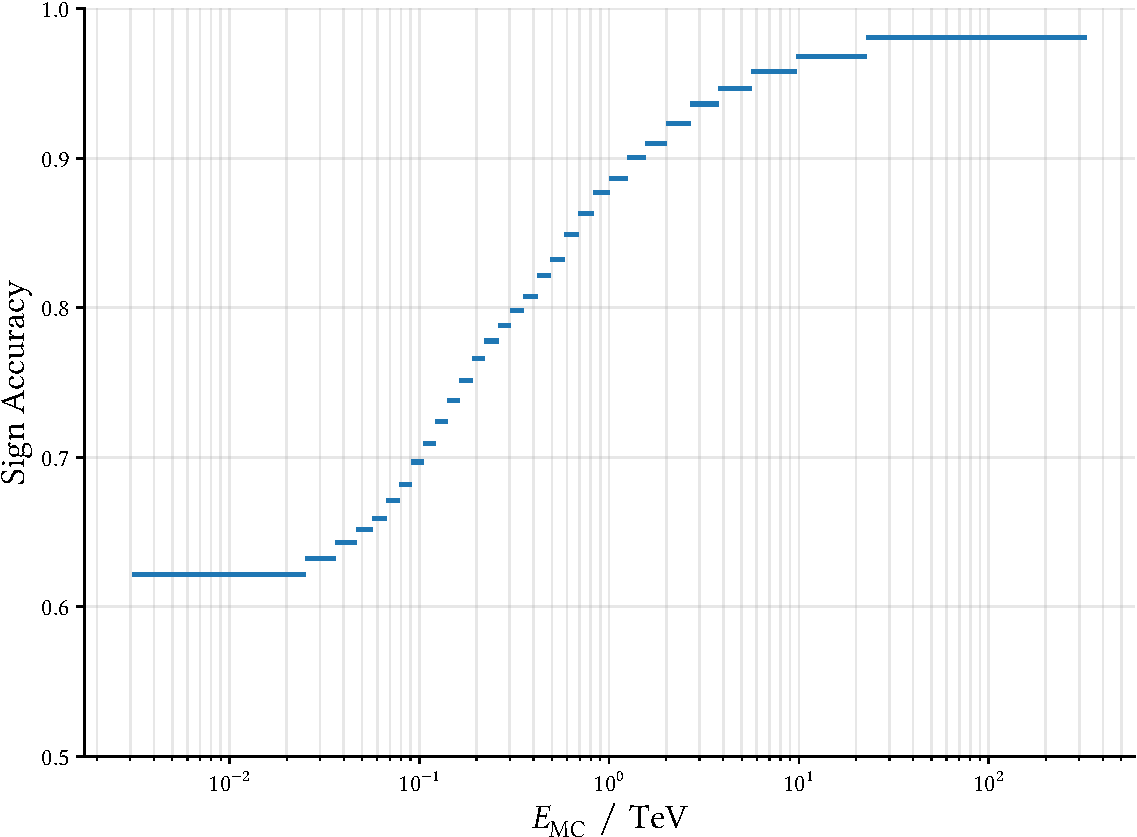
\includegraphics[width=0.9\linewidth]{../analysis/plots/disp_gamma_acc_equal_filled.pdf}
        \caption{SIGN-accuracy}
    \end{subfigure}
    \caption{Performance of the DISP- and SIGN-estimation algorithm on the pointlike dataset..}
    \label{fig:disp_gamma_perf}
\end{figure}

From figure \ref{fig:disp_features} we can learn that 
the stereoscopic features "$distance_to_reconstructed_core_position$"
and $h_max$ have a high influence on the prediction.


\begin{figure}
	\centering
	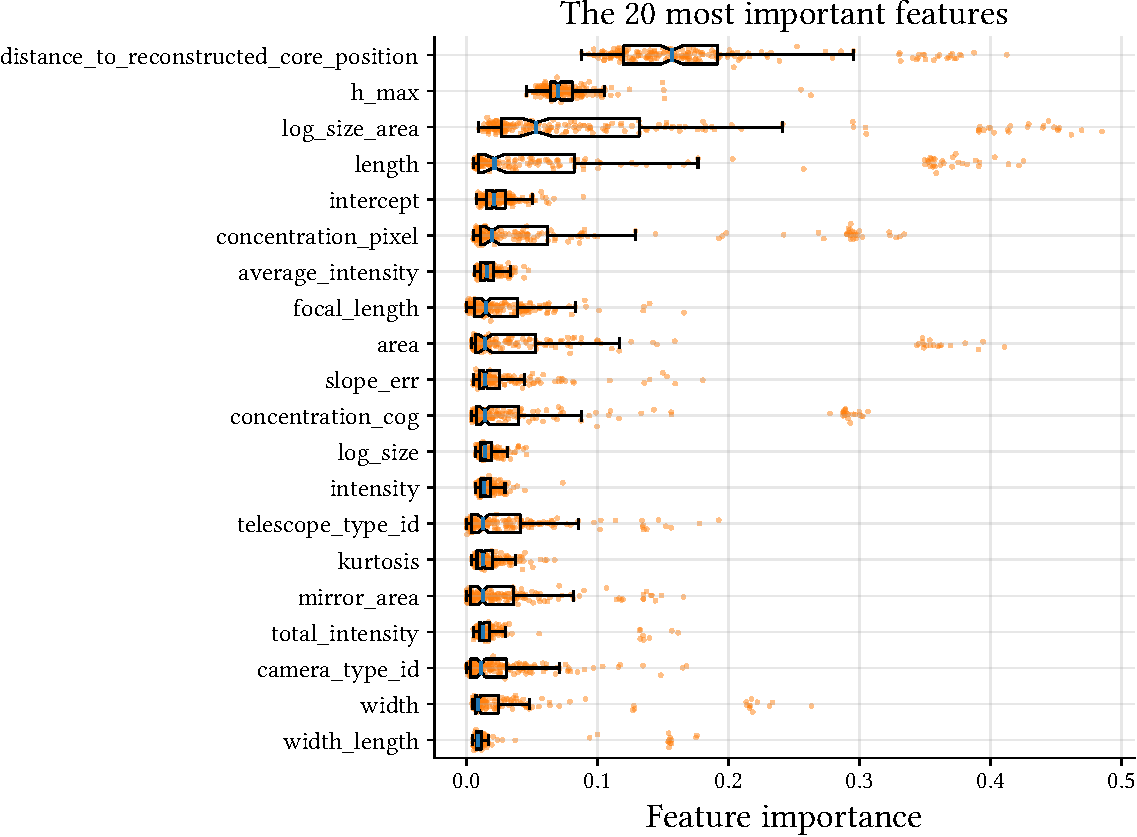
\includegraphics[width=0.8\textwidth]{../analysis/plots/disp_features.pdf}
	\caption{disp features}
	\label{fig:disp_features}
\end{figure}

The final results can be seen in figure \ref{fig:sens_telescope}.
One can derive - in accordance to the previously discussed metrics - 
that the DISP-prediction improves with increasing energies and there are less
missclassified SiGNs at higher energies.
We can also see the saturated DISP-performance at \SI{1}{\tera\electronvolt}.

\begin{figure}
    \centering
    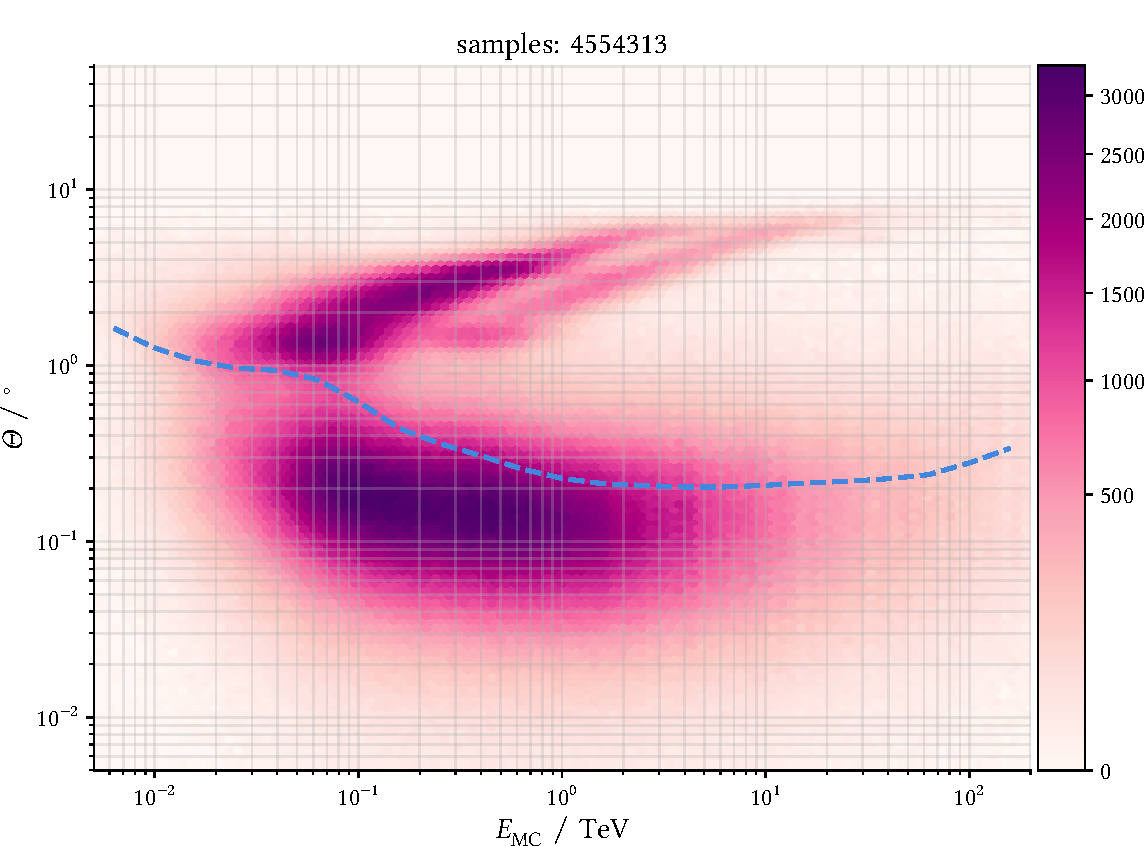
\includegraphics[width=.8\textwidth]{../analysis/plots/gamma/tel_vs_energy.pdf}
    \caption{Per telescope predictions for the source position}
    \label{fig:sens_telescope}
\end{figure}


\subsection{Analysis for the stereoscopic array}

As a baseline comparison we compare the median DISP-prediction 
with the results obtained with the Hillas-reconstructor.
These results can be seen in figure \ref{fig:stereo_double_median}.
At each energy the Hillas-reconstructor performs considerably better.
One can also see that the median predictions do not improve considerably after
\SI{3}{\tera\electronvolt} and gets worse after \SI{20}{\tera\electronvolt}.
The Hillas-reconstructor shows a similar bump at the highest energies,
so these are probably just some bad events.
It also has a short bump in the range of \SI{200}{\giga\electronvolt}
to \SI{1}{\tera\electronvolt}. This is due to a lot of multi 3 events there.
do we have a paper?

Looking at the multiplicity we can conclude that the median predictions
do not scale as well with higher multiplicities.

\begin{figure}
    \centering
    \begin{subfigure}{0.45\textwidth}
        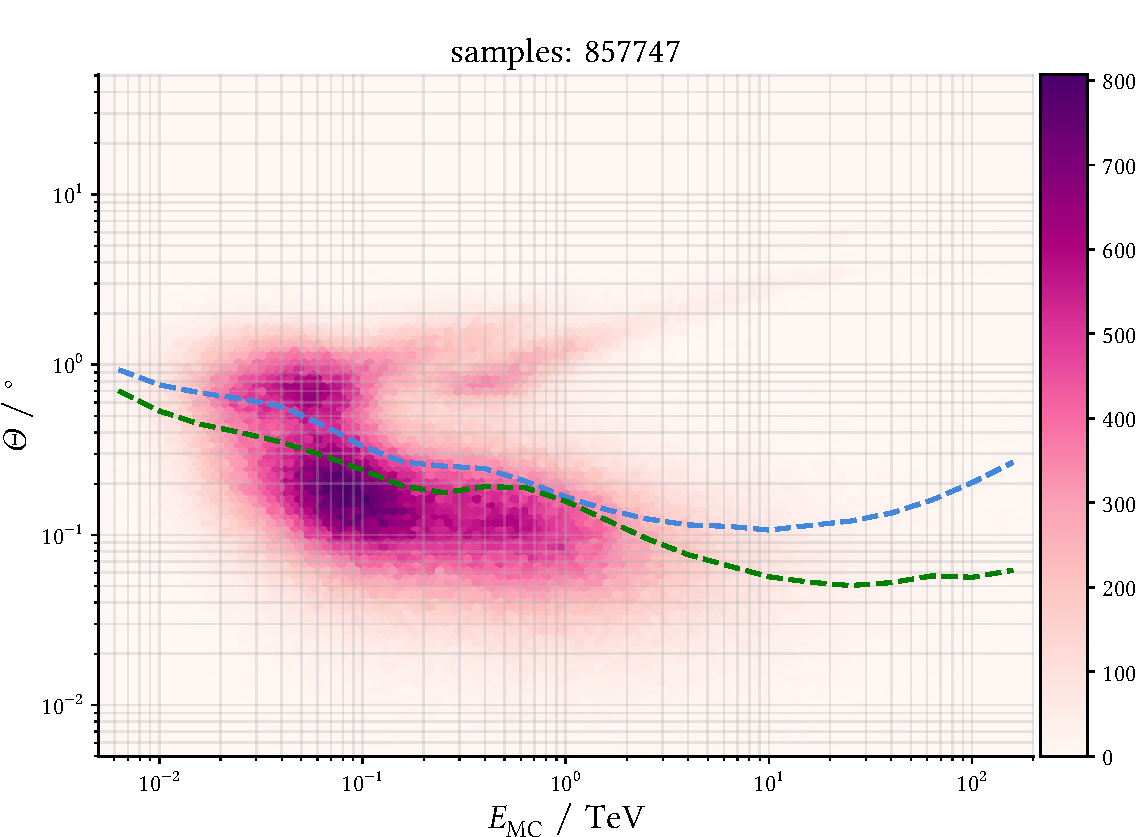
\includegraphics[width=0.9\linewidth]{../analysis/plots/gamma/median_vs_energy.pdf} 
        \caption{Distance in degree against energy}
    \end{subfigure}
    \begin{subfigure}{0.45\textwidth}
        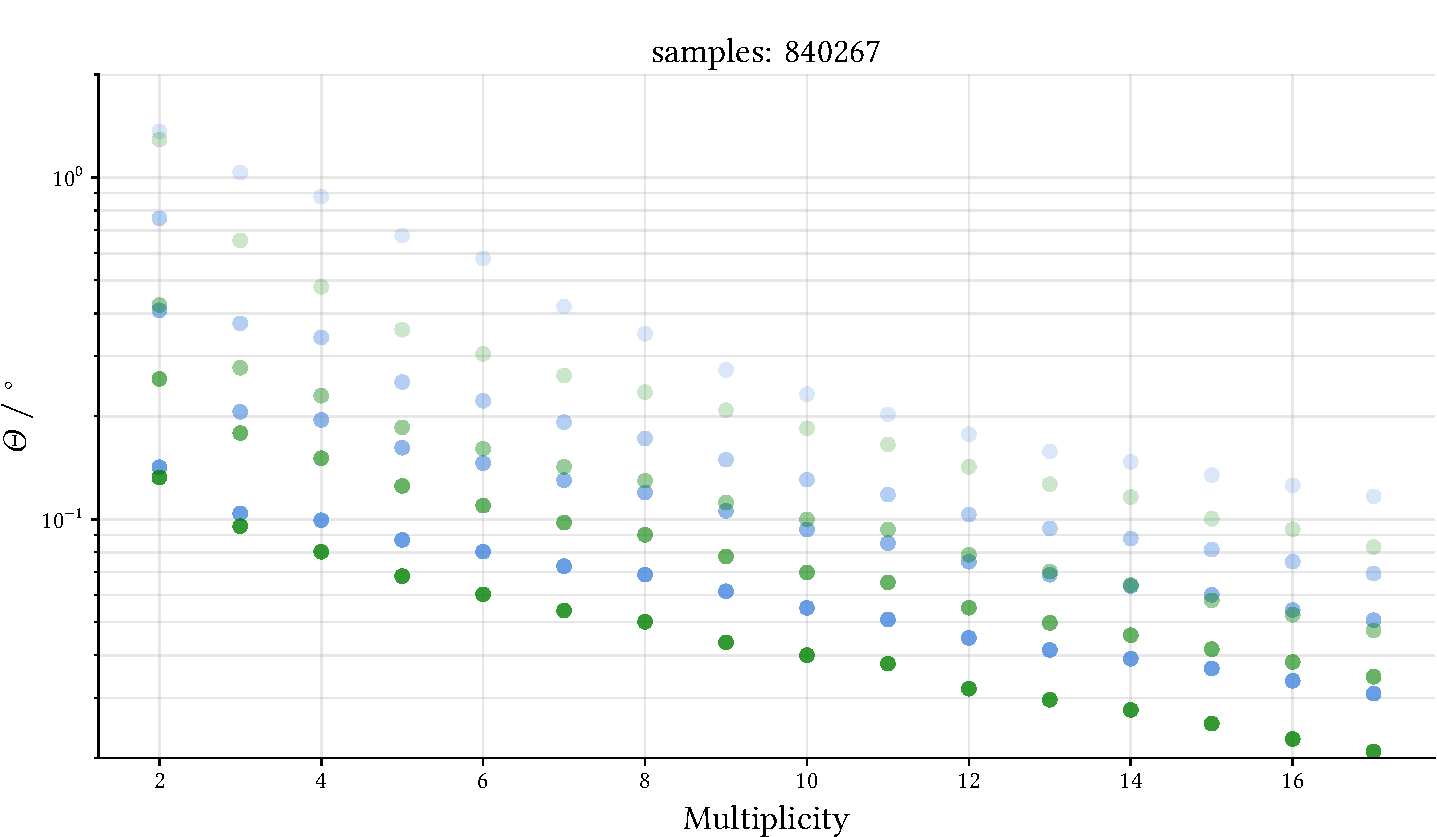
\includegraphics[width=0.9\linewidth]{../analysis/plots/gamma/median_vs_multi_comp.pdf}
        \caption{Distance in degree against multiplicity}
    \end{subfigure}
    \caption{Performance of the median telescope prediction compared 
    against the Hillas-Reconstructor. Median in Blue, Hillas in green. bins from median, hillas
    line extra}
    \label{fig:stereo_double_median}
\end{figure}

The results of the more sophisticated DISP-approach can be seen in figure \ref{fig:stereo_double_magic}.
Compared to figure \ref{fig:stereo_double_median} the completely misreconstructed events are almost
gone and the 68\% percentile is much improved throughout the complete energy range despite 
the very highest energies. At this point the DISP-error is probably limiting and the 
Hillas-reconstructor leads to much better results.
At the lower energy range our approach seems to be working pretty well, 
slightly outperforming the Hillas-reconstructor.
When looking at the multiplicity-plot, we see a similar picture as before but with 
better results. At high multiplicities $\ge 3$ the Hillas-reconstructor 
leads to better results. Improvements can be seen especially at 2-multiplicity 
events. In that case the iterative approach is identical to the 
base Magic-method.
The Hillas-reconstructor on the other hand does not work too well with 2 
triggered telescopes, with 3 triggered telescopes leading to much better results 
already.


\begin{figure}
    \centering
    \begin{subfigure}{0.45\textwidth}
        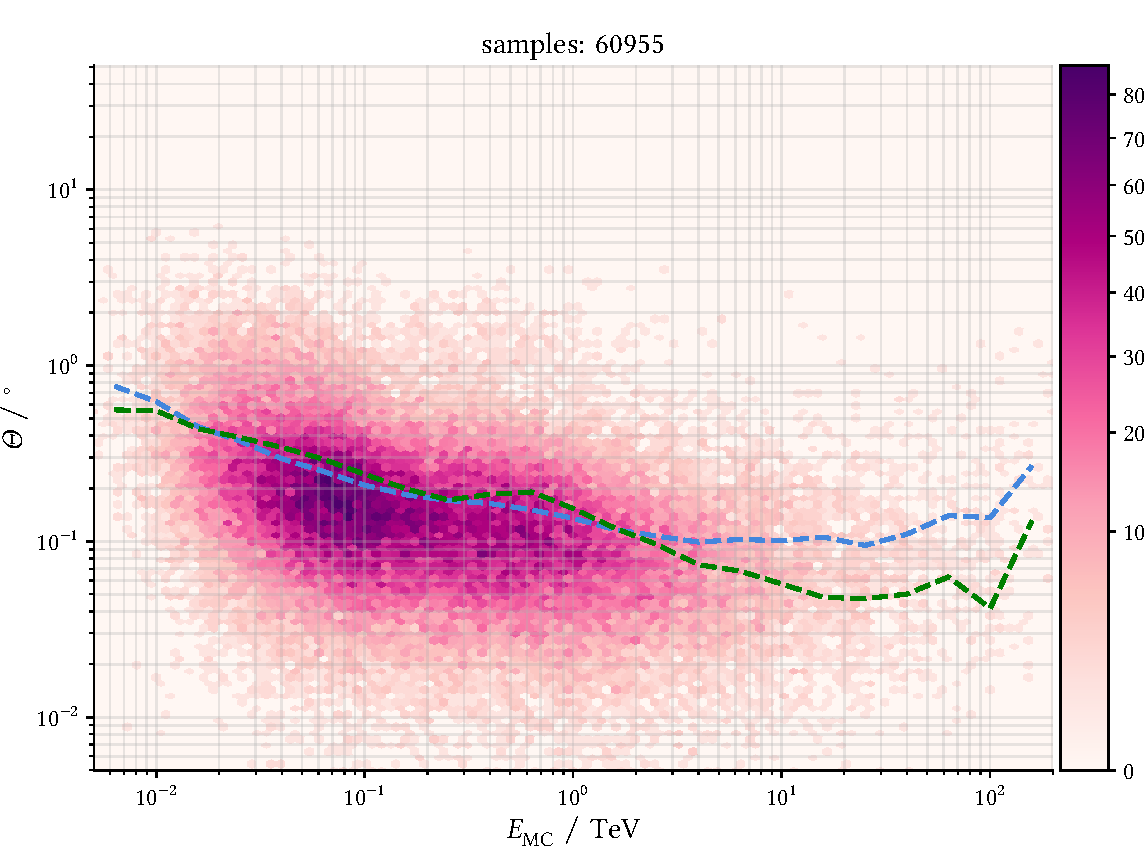
\includegraphics[width=0.9\linewidth]{../analysis/plots/gamma/pairwise_median_100_vs_energy.pdf} 
        \caption{Distance in degree against energy}
    \end{subfigure}
    \begin{subfigure}{0.45\textwidth}
        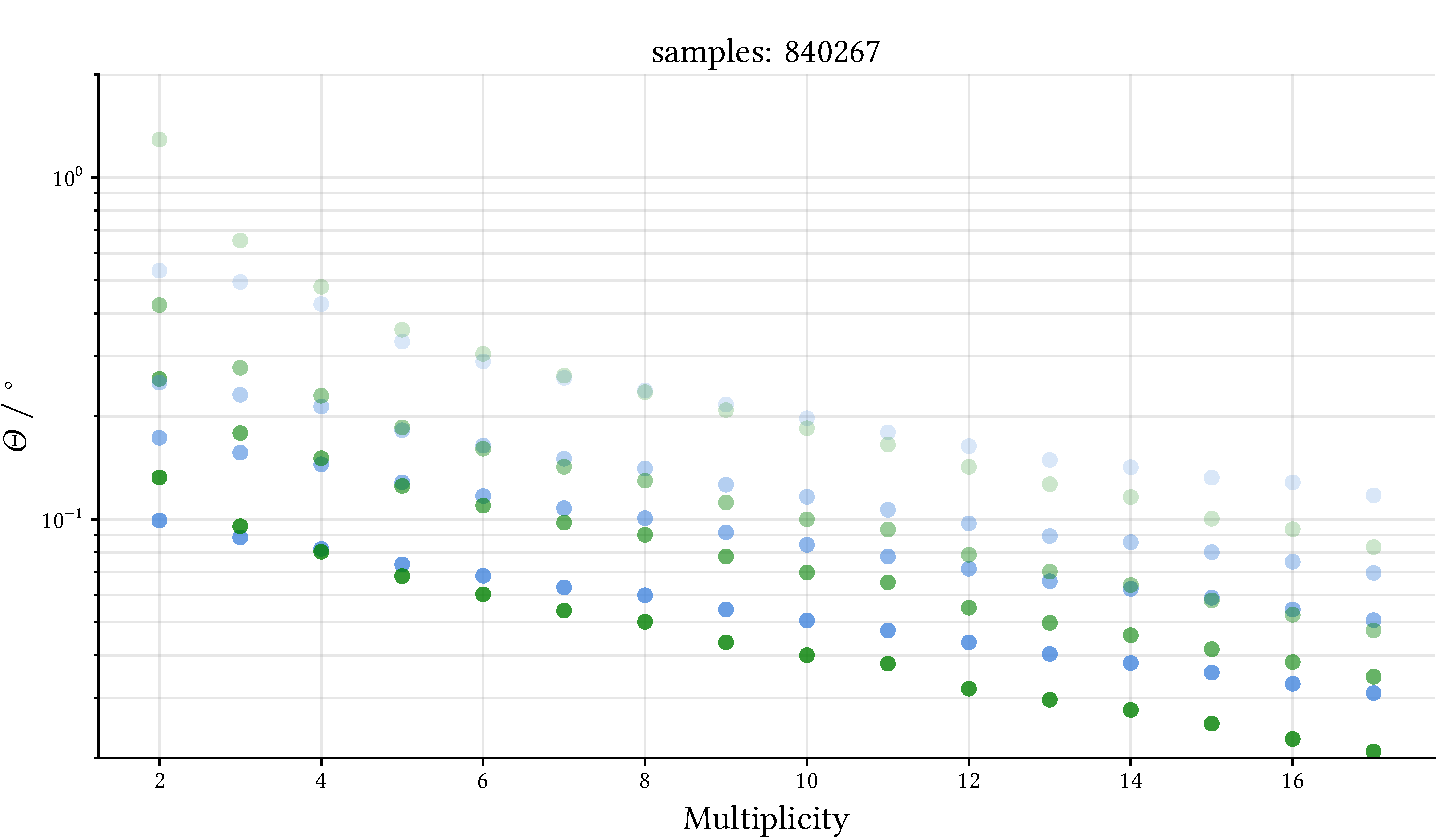
\includegraphics[width=0.9\linewidth]{../analysis/plots/gamma/pairwise_median_100_vs_multi_comp.pdf}
        \caption{Distance in degree against multiplicity}
    \end{subfigure}
    \caption{Performance of the superduper compared 
    against the Hillas-Reconstructor. Median in Blue, Hillas in green
    Actually better, but in the extreme regions where statistics is low as well.}
    \label{fig:stereo_double_magic}
\end{figure}


\section{hadroness cut}

In a analysis of real data, some legitimate events usually get discarded
in the gamma-/hadron-separation step.
Assuming that the misclassified events are in some way non regular, it might be 
justified to assume that these events also behave abnormal during the reconstruction of 
the source position. Discarding these events could thus improve the overall 
predictions.

The predictions of the gamma-/hadron-separation model on the cross-validated dataset
are summarized in figure \ref{plot aus aict tools!}.
Based on this performance we set the gammaness cut at XXX.


With this cut XXX events remain.
\begin{figure}
    \centering
    \begin{subfigure}{0.45\textwidth}
        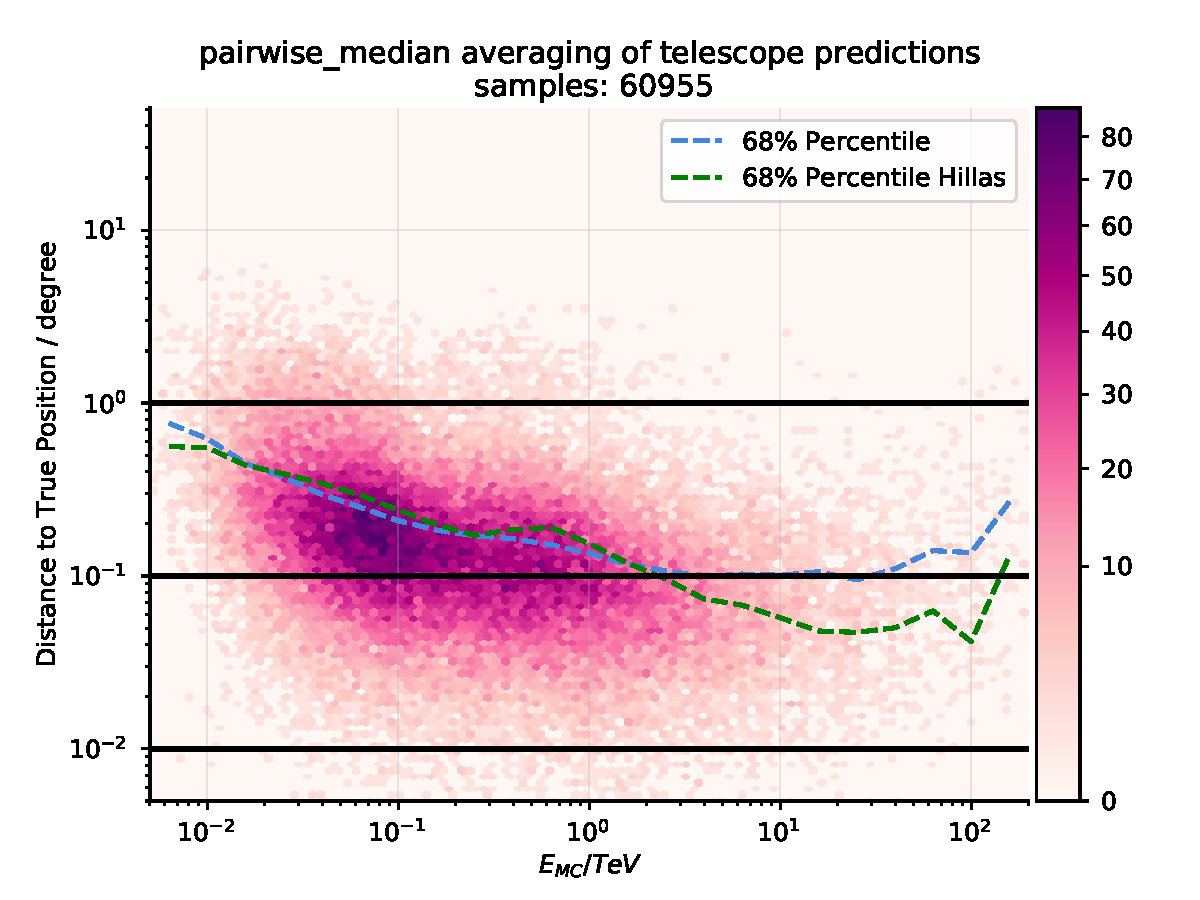
\includegraphics[width=0.9\linewidth]{../analysis/plots/gamma_cut/pairwise_median_100_vs_energy.pdf} 
        \caption{Distance in degree against energy}
    \end{subfigure}
    \begin{subfigure}{0.45\textwidth}
        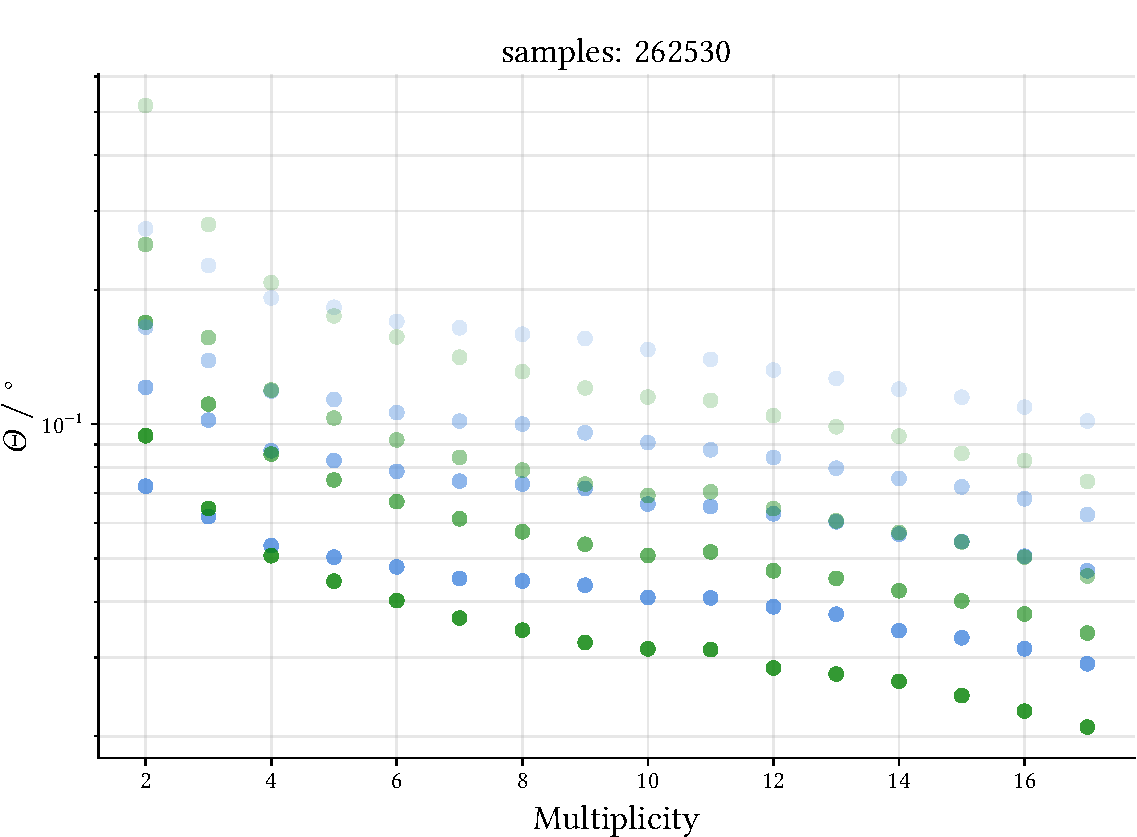
\includegraphics[width=0.9\linewidth]{../analysis/plots/gamma_cut/pairwise_median_100_vs_multi_comp.pdf}
        \caption{Distance in degree against multiplicity}
    \end{subfigure}
    \caption{Performance of the superduper compared 
    against the Hillas-Reconstructor. Median in Blue, Hillas in green
    Actually better, but in the extreme regions where statistics is low as well.}
    \label{fig:stereo_double}
\end{figure}


-> bringt nichts?


\section{LST only}
To simulate early operation stages where the LST1 is the only fully functional 
telescope, the analysis is limited to only the single LST with 
the simtel id 4.

This means that we do not have a baseline Hillas Reconstructor as we can not use
stereoscopy and each array event holds exactly one telescope event.
We expect to
get a similar sensitivity as in the earlier figure \ref{fig:sens_telescope}.

We also limit the training data, so we will have trained on less samples as well.

HOW DOES THE PERFORMANCE CHANGE?
THIS REQUIRES MORE EVENTS AND MAYBE MORE LSTS FOR TRAINING?

\begin{figure}
    \begin{subfigure}{0.45\textwidth}
        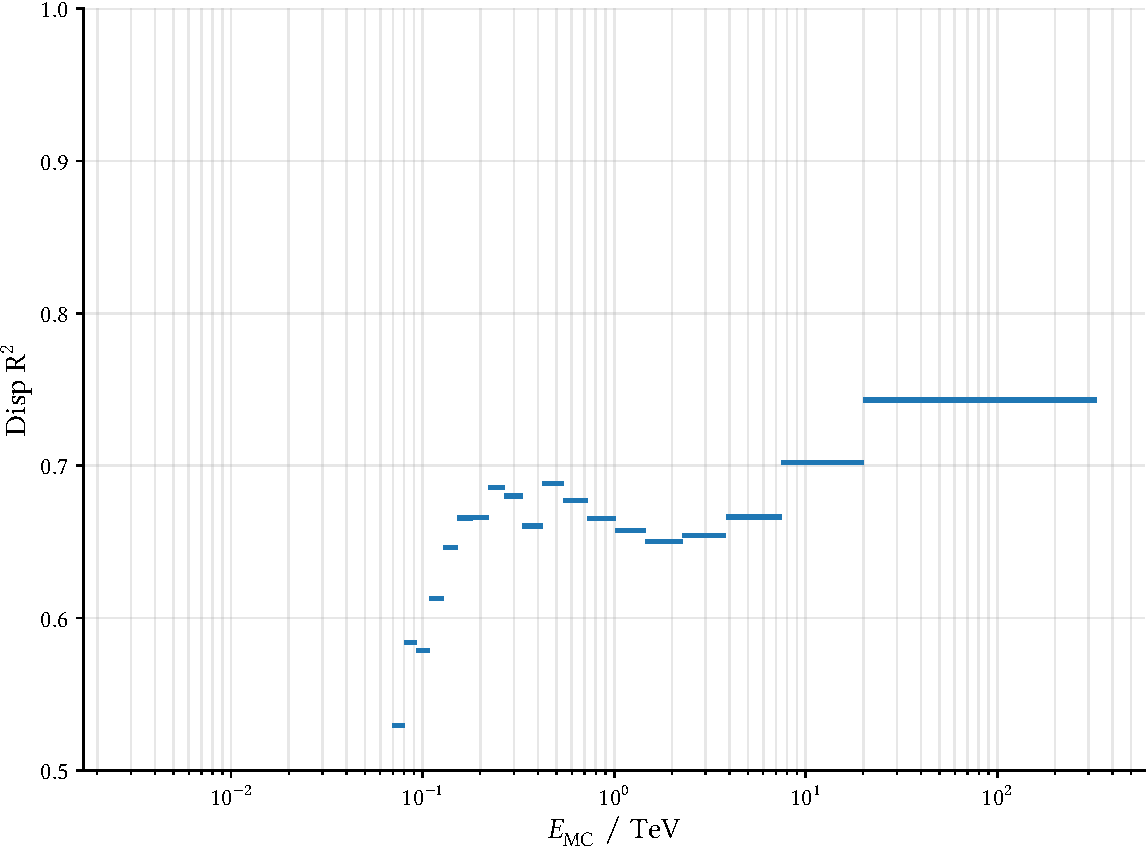
\includegraphics[width=0.9\linewidth]{../analysis/plots/disp_test_mono_lst_r2_equal_filled.pdf} 
        \caption{R2-Score for the DISP-estimation}
    \end{subfigure}
    \begin{subfigure}{0.45\textwidth}
        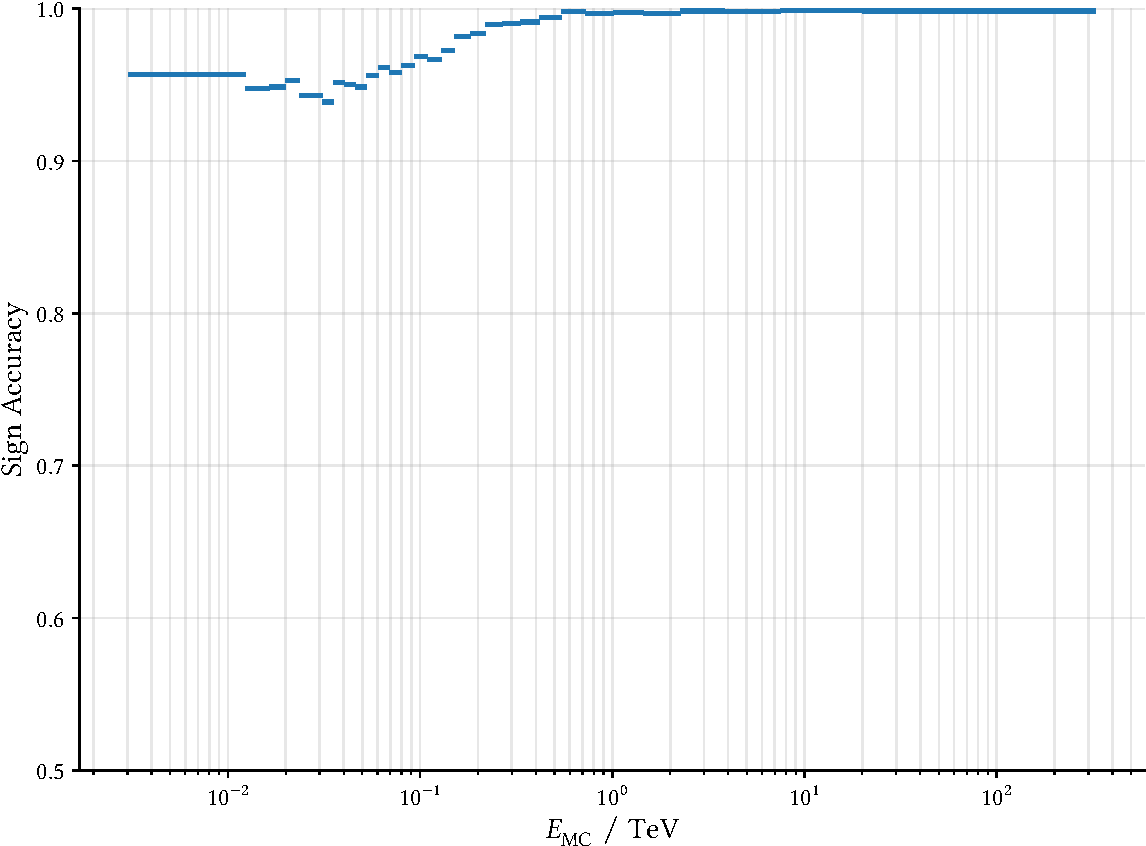
\includegraphics[width=0.9\linewidth]{../analysis/plots/disp_test_mono_lst_acc_equal_filled.pdf}
        \caption{SIGN-accuracy}
    \end{subfigure}
    \caption{Performance of the DISP- and SIGN-estimation algorithm on the test-dataset.}
    \label{fig:disp_test_perf}
\end{figure}

\begin{figure}
    \begin{subfigure}{0.45\textwidth}
        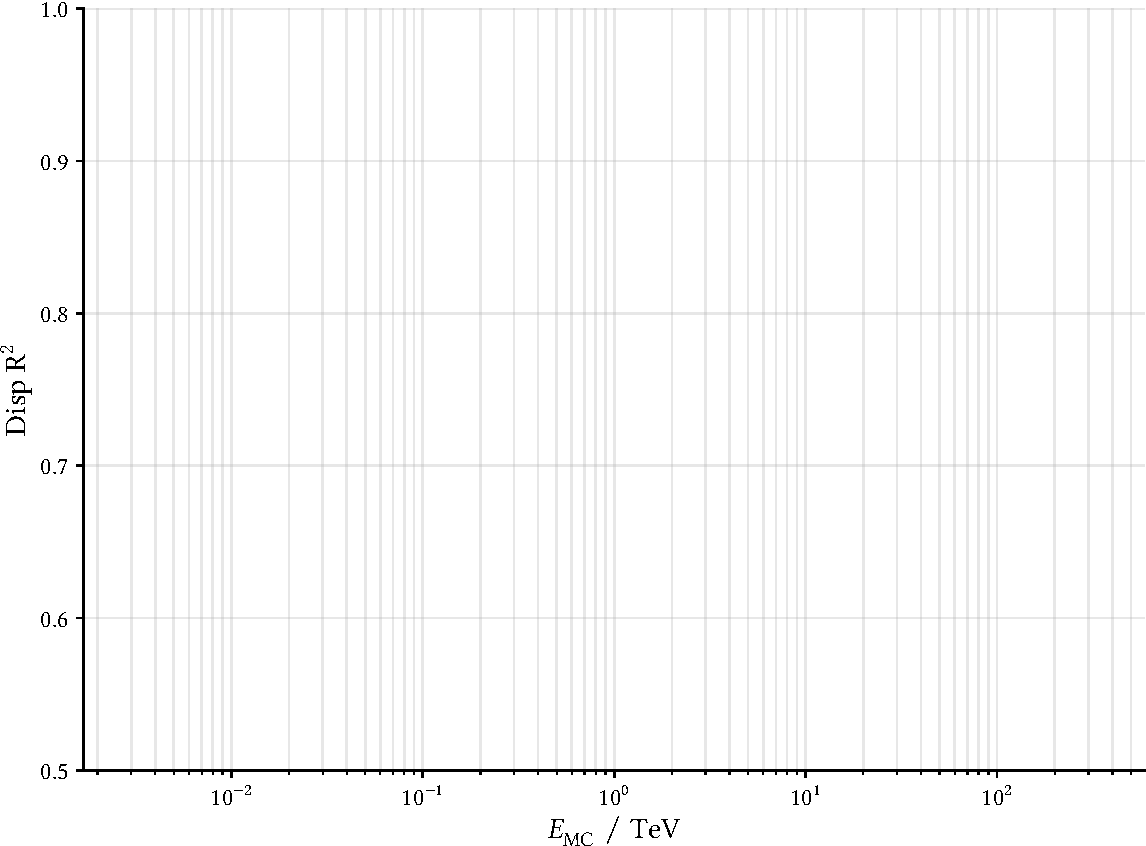
\includegraphics[width=0.9\linewidth]{../analysis/plots/disp_gamma_mono_lst_r2_equal_filled.pdf} 
        \caption{R2-Score for the DISP-estimation}
    \end{subfigure}
    \begin{subfigure}{0.45\textwidth}
        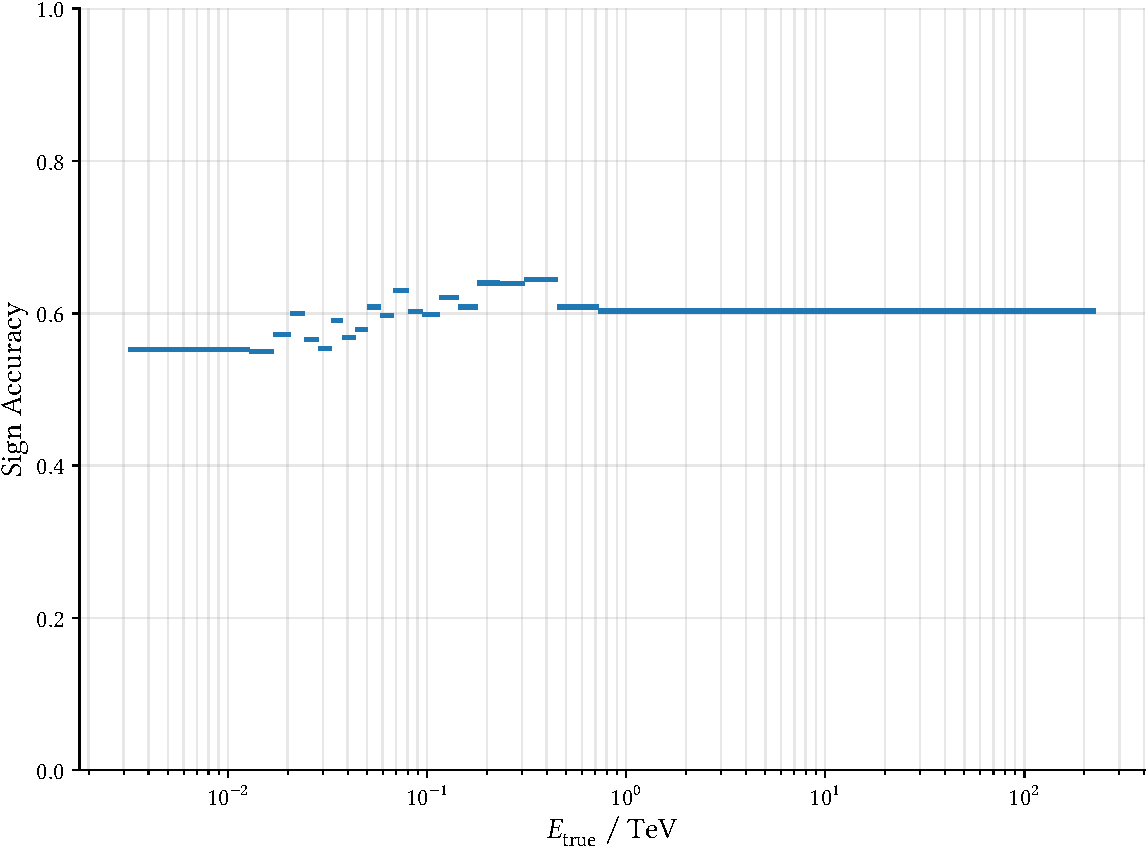
\includegraphics[width=0.9\linewidth]{../analysis/plots/disp_gamma_mono_lst_acc_equal_filled.pdf}
        \caption{SIGN-accuracy}
    \end{subfigure}
    \caption{Performance of the DISP- and SIGN-estimation algorithm on the pointlike dataset..}
    \label{fig:disp_gamma_perf}
\end{figure}

Looks decent, energy obviously limited bc LST.
